\documentclass[12pt,a4paper]{article}
\usepackage[margin=2cm]{geometry}
\usepackage{tikz}
\usepackage{multicol}
\usepackage{enumitem}
\usepackage{titlesec}
\usepackage{helvet}
\renewcommand{\familydefault}{\sfdefault}

\titleformat{\section}{\Large\bfseries}{}{0em}{}

\begin{document}

\begin{center}
    \LARGE\textbf{Cartão-Resposta – Avaliação AT1: Matemática}
\end{center}
\vspace{0.5cm}

% Informações do estudante
\noindent
\textbf{Estudante:} \rule{10cm}{0.4pt} \\[0.3cm]
\textbf{Série/Turma:} \rule{4.5cm}{0.4pt} \hfill
\textbf{Componente Curricular:} \rule{5cm}{0.4pt} \\[0.3cm]
\textbf{Professor(a):} \rule{8cm}{0.4pt} \hfill
\textbf{Total de Acertos:} \rule{2cm}{0.4pt} \\

\vspace{0.5cm}
\hrule
\vspace{0.5cm}

% Questões e alternativas
\section*{Respostas}

\newcommand{\questao}[1]{
    \noindent\textbf{#1)} 
    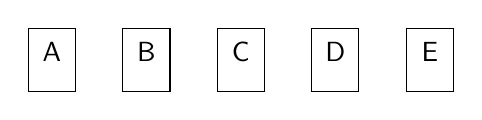
\begin{tikzpicture}[baseline={(0,-0.3)}]
        \foreach \i/\letra in {0/A,1/B,2/C,3/D,4/E} {
            \node at (\i*1.2, 0) {\letra};
            \draw (\i*1.2-0.3, -0.5) rectangle (\i*1.2+0.3, 0.3);
        }
    \end{tikzpicture}
    \vspace{0.4cm}
}

\begin{multicols}{2}
    \questao{01}
    \questao{02}
    \questao{03}
    \questao{04}
    \questao{05}
    \questao{06}
    \questao{07}
    \questao{08}
    \questao{09}
    \questao{10}
\end{multicols}

\vfill
\hrule
\vspace{0.3cm}
\noindent\small\textit{Assinatura do(a) estudante:} \rule{8cm}{0.4pt}
\hfill
\textit{Data:} \rule{3cm}{0.4pt}

\end{document}

